\chapter{満足性と容積脈波から得るストレス指標との関係性}
\label{chap:pulsewave}

本章では,後述の時系列UX評価システムの開発に先立ち,容積脈波によるストレス指標と満足性の関連を把握するために行った予備実験について述べる.新たなストレス指標としては自律神経バランス(ANB)と最大リヤプノフ指数(LLE)を検討した.

\section{実験方法}

実験では,Nielsenのヒューリスティクスに基づいて作成した2つのUIを使ったタスクを被験者に実施してもらい,それぞれを使用している際のANBとLLEを比較した.ヒューリスティクスでBad UIとされているものは多くの場合満足性が低くなると考えられるものの,はユーザビリティ評価に使用するものであり,それがそのまま満足性に直結するとはいえない.そこで自己申告メトリクスを併用し,どちらのUIがより好ましかったかについて回答を求めた.

実験は2020年3月に17歳から74歳までの10名(男性8名,女性2名)を対象に行った.

\subsection{実験マテリアルの開発}

UX評価のマテリアルとして,Nielsenのヒューリスティクスで推奨されているUI(Good UI)と避けるべきとされているUI(Bad UI)を用意した.今回対象としたヒューリスティクスは``Visibility of system status'’(システムの状態の可視性)\cite{nielsen1990} である.10のヒューリスティクスのなかでアプリケーションの機能に関係ないものや学習が必要なもの,ユーザの予備知識に関係するものなど今回の実験に適さないものを排除して選択した.

具体的にはプログレス表示があるものをGood UI,無いものをBad UIとした.マテリアルの画面は図\ref{fig:old1}の通りである.画面にはノイズにならないように数字を表示するラベルと数字を変更するボタンのみを配置した.また,右上のスイッチでスタッフがGood UIとBad UIを切り替えられるようにした.アプリケーションの機能はNEXTボタンをタップするとランダムで0-5秒後にランダムな数字の表示が切り替わるだけのシンプルなものである.Good UIではNEXTボタンをタップすると図\ref{fig:old2}のようにプログレスを表示するインジケータが表示され,システムが次の数字を読み込み中であるという状態を表示する.一方でBad UIではNEXTボタンを押してもその時点では何の反応もなく,0-5秒後に数字が切り替わるまで上手くタップできたかどうかがわかりにくくなっている.

\begin{figure}[htbp]
  \begin{minipage}{0.5\hsize}
    \begin{center}
       \fbox{
\includegraphics[width=40mm]{img/old1.png}}
    \end{center}
    \caption{実験マテリアル:数字の表示画面}
    \label{fig:old1}
  \end{minipage}
  \begin{minipage}{0.5\hsize}
    \begin{center}
       \fbox{
\includegraphics[width=40mm]{img/old2.png}}
    \end{center}
    \caption{実験マテリアル:数字の読込中画面}
    \label{fig:old2}
  \end{minipage}
\end{figure}

\subsection{タスクの実施}
被験者にマテリアルを操作してもらう際には,バイアスがかからないようにダミータスクを用意したうえでGood UIとBad UIそれぞれを順番に実施してもらった.なお,Good UIとBad UIの間には3分間の安静時間を設け,それぞれのマテリアルを操作する順番はカウンターバランスをとった.

ダミータスクは,1分間でNEXTボタンをタップして表示される数字をできるだけ多く書き取るものにした.できるだけ多く書くようにと指示することで,競争意識によって手を抜きにくくなるほか,早く表示してほしいと思わせるように設計した.

\begin{itembox}[l]{タスクの指示}
\begin{verbatim}
今から1分間のテストを2回行ってもらいます.このアプリでは,NEXTボタンを押すと数字が読み込まれますので紙に表示された数字を書いてください.書き終わったらもう一度NEXTボタンを押して次の数字を読み込んで紙に書いてください.制限時間は1分ですのでできるだけ沢山書くようにしてください.ただし,NEXTボタンを押してから数字が読み込まれるまで少し時間がかかりますので待ってください.
\end{verbatim}
\end{itembox}

\subsection{容積脈波(BVP)の計測}
BVPの計測は光学式指尖容積脈波計(PPG)のLifescore Quickプローブ(型番LQ-11,図\ref{fig:device2} )と専用の分析システムであるLyspect\cite{chaotechlyspect}を使用した.Lyspectでは300HzでBVPを記録し,LLEの平均とHF及びLFの値を取得した(図\ref{fig:lyspect}).被験者には実験の開始から終了まで利き手と逆の人差し指にセンサを装着してもらい休憩中も外さないようにした.なお,計測はマテリアルを使用している1分間の間のみとし1人当たり計2回記録した.


\begin{figure}[htbp]
  \begin{minipage}{\hsize}
    \begin{center}
       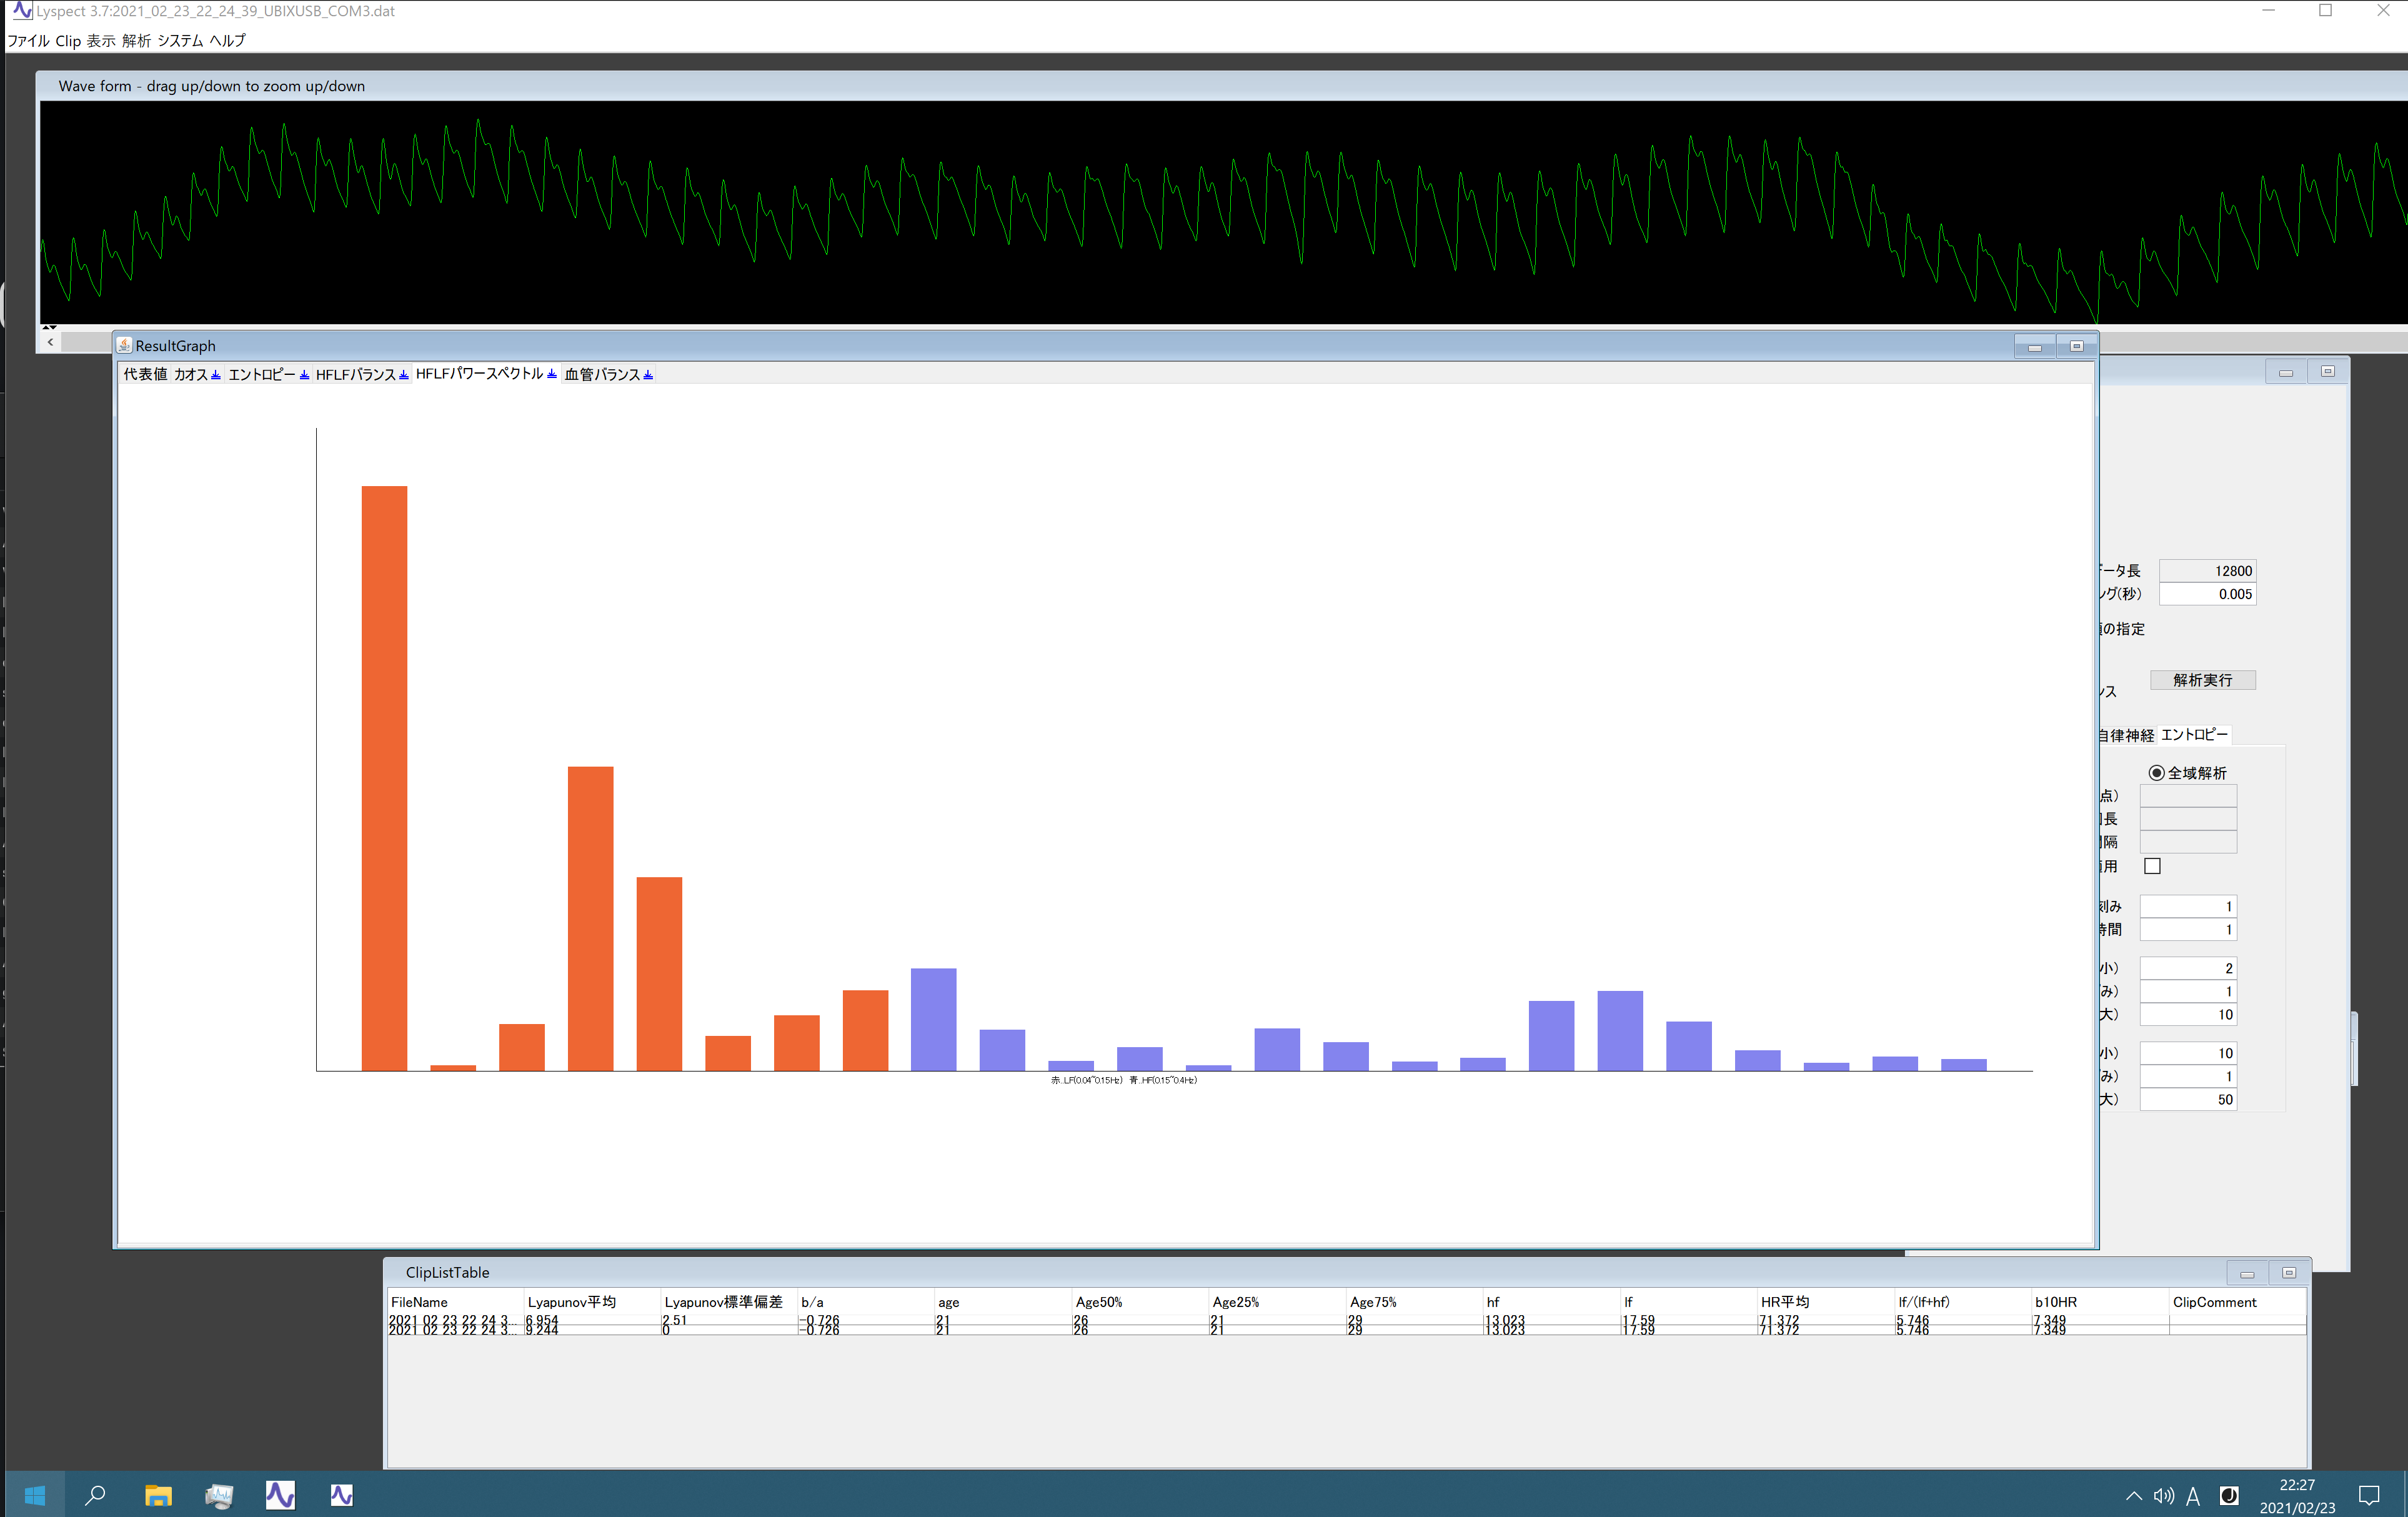
\includegraphics[width=100mm]{img/lyspect.png}
    \end{center}
    \caption{Lyspectでの分析画面}
    \label{fig:lyspect}
  \end{minipage}
\end{figure}


\section{結果}

\section{考察}

